% coupling_oil
In this section a different background environment is contained in the coupling simulation. For the practical experiment there are no many options for changing the environment. Here the coupling configuration in section \ref{sect:model_model_fiber2chip} will be placed in an environment full of oil. Changing the background may greatly affect the working distance of the  TLF. Therefore determining the new working distance is necessary before couple the TLF to the waveguide.  Similar as in section \ref{sect:model_model_model_TLF} the spot size curve Fig. \ref{fig:oil_spot_curve} can be drawn by loading data from the simulation of TLF beam propagation in oil. Here we can tell from the spot size cure that the minimum spot in oil lies at the position farmer than the original minimum spot in air.    
\begin{figure}[!ht]
\centering
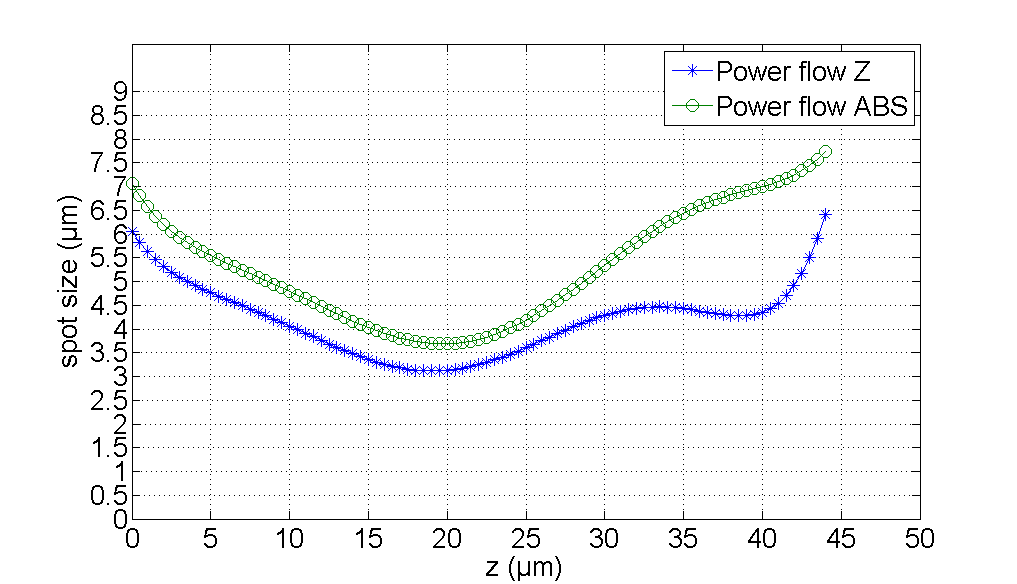
\includegraphics[width=0.7\textwidth]{bilder/spot_curve_oil}
\caption{Spot size curve of TLF in oil.}
\label{fig:oil_spot_curve}
\end{figure}
Place the waveguide at the new working distance and execute the coupling simulation. The coupling efficiency of Fiber-to-Chip in oil can be found in curve Fig. \ref{fig:oil_coupling_curve}. The result shows that the coupling efficiency at working frequency $282$THZ achieves about $34.5\%$, which is lower than that of the original configuration in section \ref{sect:model_model_model_TLF}.
\begin{figure}[!ht]
\centering
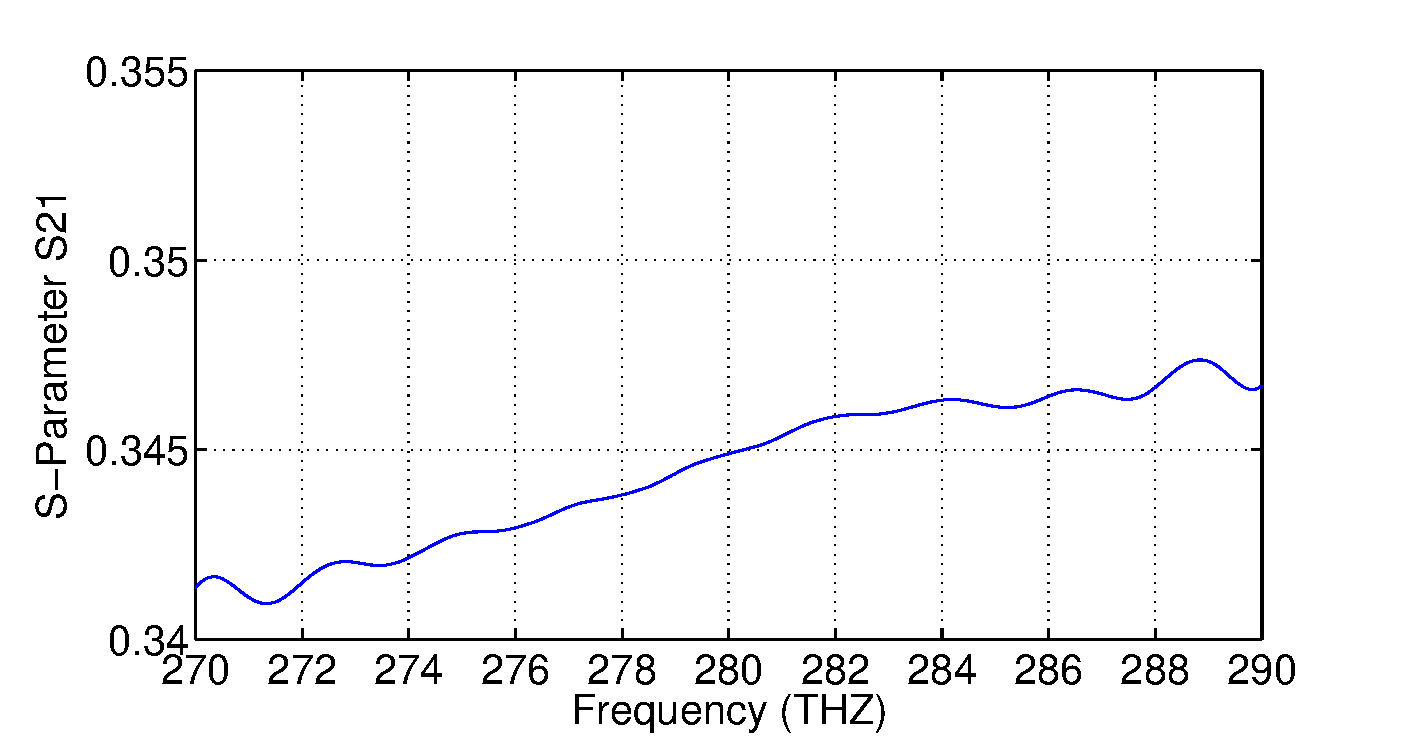
\includegraphics[width=0.7\textwidth]{bilder/s21_oil_curve}
\caption{Coupling efficiency between TLF and the rib waveguide due to frequency domain in oil background.}
\label{fig:oil_coupling_curve}
\end{figure}
